\documentclass[11pt]{article}
\usepackage[utf8]{inputenc}
\usepackage[T1]{fontenc}
\usepackage{fixltx2e}
\usepackage{graphicx}
\usepackage{longtable}
\usepackage{float}
\usepackage{wrapfig}
\usepackage{rotating}
\usepackage[normalem]{ulem}
\usepackage{amsmath}
\usepackage{textcomp}
\usepackage{marvosym}
\usepackage{wasysym}
\usepackage{amssymb}
\usepackage[hidelinks]{hyperref}
\usepackage{listings}
\usepackage{xcolor}


\lstdefinestyle{customc}{
  belowcaptionskip=1\baselineskip,
  breaklines=true,
  frame=L,
  numbers=left,
  stepnumber=1,
  tabsize=4,
  xleftmargin=\parindent,
  language=C,
  showstringspaces=false,
  basicstyle=\footnotesize\ttfamily,
  keywordstyle=\bfseries\color{green!40!black},
  commentstyle=\itshape\color{purple!40!black},
  identifierstyle=\color{blue},
  stringstyle=\color{orange},
}

\lstdefinestyle{customasm}{
  belowcaptionskip=1\baselineskip,
  frame=L,
  xleftmargin=\parindent,
  language=[x86masm]Assembler,
  basicstyle=\footnotesize\ttfamily,
  commentstyle=\itshape\color{purple!40!black},
}

\lstset{escapechar=@,style=customc}


\author{Sizhe Yuen}
\title{CS4052 Logic and Software Verification}

\begin{document}

\maketitle
\tableofcontents

\newcommand{\n}[0]{\\[\baselineskip]}

\section{Introduction}


\section{Preliminaries}

\subsection{Characteristics of Model Checking}
A system model can be simulated with formal methods. Violations in the model will give counterexamples of the error in the software logic. There are a few typical properties we want to check for.
\begin{itemize}
\item Is the generated result correct (value within bounds)?
\item Does the system terminate correctly?
\item Can the system reach a \textbf{deadlock} situation?
\item Can a deadlock occur at a certain point in the system?
\item Is a response always received after some time?
\end{itemize}

\begin{figure}[H]
\centering
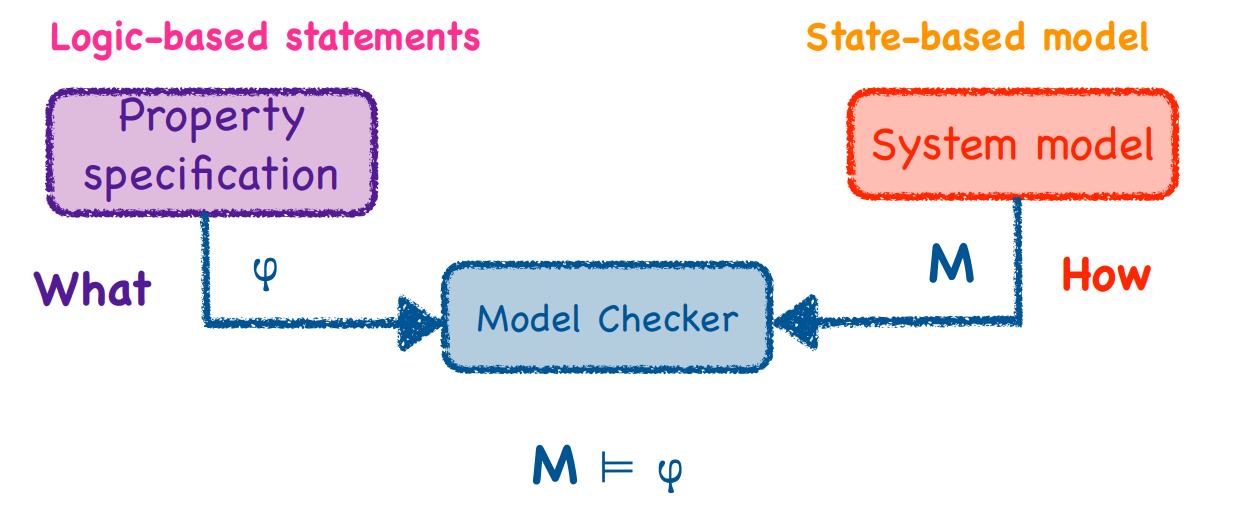
\includegraphics[width=1\textwidth, keepaspectratio]{imgs/model-checker-logic.png}
\caption{High level idea of a what a model checker does.}
\end{figure}
\noindent
The model checker examines all relevant states in M to check if $\phi$ is satisfied. If a state is found where $\phi$ is violated, the model checker provides a counterexample as to how that state can be reached. The counterexample describes an execution path that leads from the initial state to the state that violets $\phi$. 
\n
\subsection{Concurrency and Atomicity}
Most errors in models are classic \textbf{concurrency errors}. This is where unforeseen interleavings between processes caused issues such as deadlock or changing state when the model isn't supposed to. Wrong assumptions are often made as to what is executed atomically. 
\\
\begin{lstlisting}[caption={Concurrency example in pseudocode}, captionpos=b]
proc Inc = while true do if x < 200 then x += 1
proc Dec = while true do if x > 0 then x -= 1
proc Reset = while true do if x == 200 then x = 0
\end{lstlisting}
\noindent
In the code above, x is a shared variable and all three processes depend on the value of x. Because the instructions between conditional of the \texttt{if} and the \texttt{then} are not atomic, it is possible for x to become negative when the condition of \texttt{Reset} is interleaved with the \texttt{Dec} process. 

\subsection{Temporal Logic}
\textbf{Temporal logic} is an extension of basic propositional logic using \textbf{temporal operators} that describe the behaviour of the system over time. This is useful for describing different system properties:
\begin{itemize}
\item \textbf{Functional correctness} - Does the system behave as expected?
\item \textbf{Reachability} - Is it possible to reach a deadlock state?
\item \textbf{Safety} - Something bad never happens (e.g. Two processes both in the critical section)
\item \textbf{Liveness} - Something good will eventually happen (e.g. Printer process eventually prints)
\item \textbf{Fairness} - Under certain conditions, can an event occur repeatedly?
\item \textbf{Real time properties} - Is the system acting in time?
\end{itemize}
\noindent
A classic issue for model checkers if if the model is too large to be handled. This results in a \textbf{state-space explosion} where the number of states needed to model the system accurately easily exceeds the amount of available computer memory. Different techniques must be applied to exploit regularities in the structure of the model to prevent this problem.
\section{PROMELA and SPIN}
\subsection{PROMELA}
PROMELA (PROcess MEta LAnguage) is a specification language used for model checking with a tool called \textbf{Spin}. It contains the notion of \textit{communication channels} as it was originally developed for specification of communication protocols. 
\n
PROMELA can model concurrent systems made of processes which can:
\begin{itemize}
\item Behave \textbf{independently} (interleaving)
\item Communicate indirectly using \textbf{shared global variables}
\item Communicate directly using \textbf{channels} (synchronously or asynchronously)
\end{itemize}
Here is an example of a simple PROMELA specification:
\\
\begin{lstlisting}[caption={Simple PROMELA specification}, captionpos=b]
#define N 20

int res

proctype odd() {
	int x = 1;
	do
	:: x <= N -> res = res + x;
				 x = x + 2;
	:: x > N -> break;
	od
}

proctype even() {
	int x = 0;
	do
	:: x <= N -> res = res + x;
				 x = x + 2;
	:: x > N -> break;
	od
}

init {
	res = 0;
	run odd();
	run even();
}
\end{lstlisting}
\noindent
More than one alternative in a \texttt{do} loop can be given and denoted by \texttt{::}. An alternative can only be executed if its guard passes. If there are multiple branches that pass, one is chosen non-deterministically. 
\n
Boolean conditions in the middle of code blocks until it becomes true. 
\begin{lstlisting}[caption={Boolean conditions in PROMELA}, captionpos=b]
x < 4;
x > 6;
res = 20;
\end{lstlisting}
\noindent
Here, the specification must waited until \texttt{x} is smaller than 4, then wait until \texttt{x} is greater than 5 before proceeding to assign \texttt{res}.
\n
It is possible to have an \texttt{else} guard in a do loop.
\begin{lstlisting}[caption={PROMELA Do loops in detail}, captionpos=b]
active proctype ifdo() {
	do
	:: x < 10 -> x = x + 1;
	:: (x > 0 && x < 10) -> x = x - 1;
	:: x < 9 -> x = x + 3;
	:: else -> x = x + 4;
			   break;
	od
}
\end{lstlisting}
\noindent
An \texttt{else} in a \texttt{do} block is only executed if all the other guards fail. Additionally, the \texttt{break} statement is the only way to leave a \texttt{do} loop in PROMELA.

\subsubsection{Communication channels}  
In PROMELA, two processes can communicate directly using channels.
\begin{figure}[H]
\centering
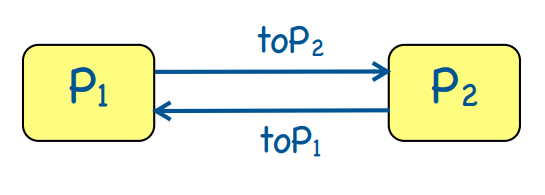
\includegraphics[width=0.6\textwidth, keepaspectratio]{imgs/promela-channels.png}
\caption{PROMELA channels.}
\end{figure}

\subsection{Linear-Time Properties}
\subsubsection{Safety Properties}
Safety properties refer to all states in the system. 
\n
Another safety property that can be checked with spin is whether at the end, all processes have reached a valid end state. A process terminates correctly if it reaches the closing bracket of its \texttt{proctype} declaration. 
\subsubsection{Liveness Properties}
Liveness properties describe the requirement that a process makes progress towards a certain goal, the achievement of which depends on the fairness of the system.  They are about something which should eventually happen. For example:
\begin{itemize}
\item \textbf{Eventually} - Each process will eventually enter its critical section. 
\item \textbf{Repeated eventually} - Each process will enter its critical section infinitely often.
\item \textbf{Starvation freedom} - Each waiting process will eventually enter its critical section.
\end{itemize}
\noindent
Liveness properties need to be checked for all possible system runs/executions. It is important to check for liveness both with and without fairness as they can tell us if the system is unfair or not by design. 
\n
Programs in spin can be annotated with labels such as:
\begin{equation*}
\text{progress}[a-zA-Z0-9_]*
\end{equation*}
\noindent
These labels are examples of a liveness property where all infinite execution paths have to pass a progress label infinitely often. There is an option in spin to tick the box for ``non-progress cycles" before running the verification.
\subsubsection{Fairness}
A \textbf{fairness constraint} is imposed on the system that it fairly selects the next process to be executed. These constraints are not a property to be verified, but they can be expressed in temporal logic to verify behaviour of a system with and without fairness constraints. Fairness assumptions are there to remove what can be considered unrealistic behaviours as it may be unrealistic for only \texttt{P1} to be executing all the time.
\n
There are different types of fairness:
\begin{itemize}
\item \textbf{Unconditional fairness} - Every process gets its turn infinitely often. This ignores that a process might not be ready to execute sometimes.
\item \textbf{Strong fairness} - Every process that is infinitely often enabled should be executed infinitely often.
\item \textbf{Weak fairness} - Every process that is always enabled from a certain point onwards should be executed infinitely often. 
\end{itemize}

\begin{figure}[H]
\centering
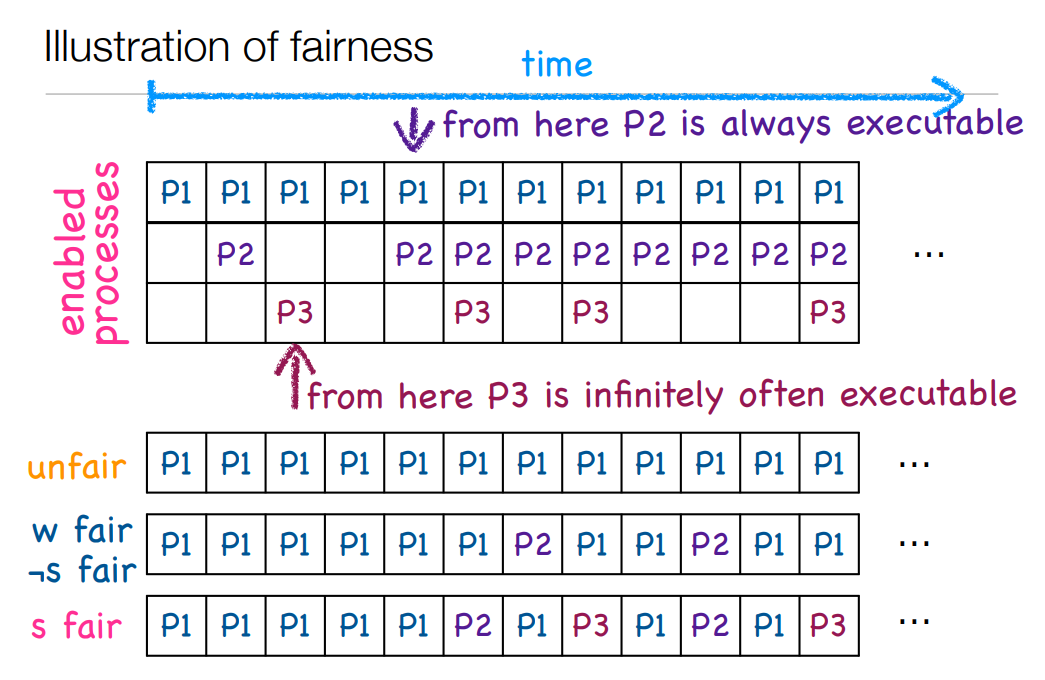
\includegraphics[width=1\textwidth, keepaspectratio]{imgs/fairness-example.png}
\caption{Illustration of different types of fairness.}

\end{figure}

\subsection{Trace constraints}
For some systems, we may want to reflect on the \textbf{patterns of communication} used. It is possible to impose sequences of communication using a \textbf{trace}. Traces have to be valid on all executions. Trace conditions are used to impose an order on the allowed sequences of communications and so \textbf{synchronises} with the specification. 
\\
\begin{lstlisting}[caption={Example of a trace in PROMELA}, captionpos=b]
mtype = {a, b};

trace {
	do
	:: c1!a;
	   c2?b;
	od
}
\end{lstlisting}
\noindent
In the example above, sending on channel \texttt{c1} alternates with receiving on channel \texttt{c2}. All messages sent on \texttt{c1} are of type \texttt{a}, and all messages received on \texttt{c2} are of type \texttt{b}. The trace here synchronises with the specified processes.
\n
Trace specifications are only concerned about \textit{communication actions} and must be deterministic. As such, each specification can only contain one trace constraint. 
\subsection{Never claims}
To check the \textit{correctness} of a specification against certain properties, it is useful to use a \textbf{never claim}. With a never claim, we are interested in the executions that \textbf{do not} satisfy the property. A never claim \textit{succeeds} (finds an error) if it terminates or it passes infinitely often through \texttt{accept} labels. It will always be executed first after global variables are initialised and before any other processes.
\n
In essence, disallowed behaviour is specified and run against the specification to check that it cannot occur. Additionally, a never claim \textit{is interleaved with the specification}. Never claims are always executed first.
\n
The issue with never claims is that it can be time consuming to construct them. They involve searching and thinking about general counter examples. An easier way would be to do the opposite and specify properties that can be used to verify that the system behaves correctly. This is \textbf{linear temporal logic} (LTL).
\section{Linear Temporal Logic}
To express properties in LTL, \textbf{atomic propositions} must first be defined:
\begin{lstlisting}[caption={Atomic propositions in PROMELA for LTL}, captionpos=b]
#define p (state == ok)
#define q (alaram != red)
\end{lstlisting}
\noindent
LTL formulae are constructed from atomic propositions combined with \textit{boolean} and \textit{temporal} operators. To be able to describe a property holding on a \textbf{state}, only propositional logic is needed. However, to describe properties about \textbf{execution} traces, temporal operators are needed.
\n
Given $p$ and $q$ are valid LTL formulae, there are the following temporal operators:
\begin{enumerate}
\item $\Box\ p$ - Always $p$
\item $\Diamond\ p$ - Eventually $p$
\item $X\ p$ - Next $p$
\item $p\ U\ q$ - $p$ Until $q$
\end{enumerate}
\noindent
Formulae can be combined with normal boolean operators such as \wedge (and), \vee (or).
\begin{figure}[H]
\centering
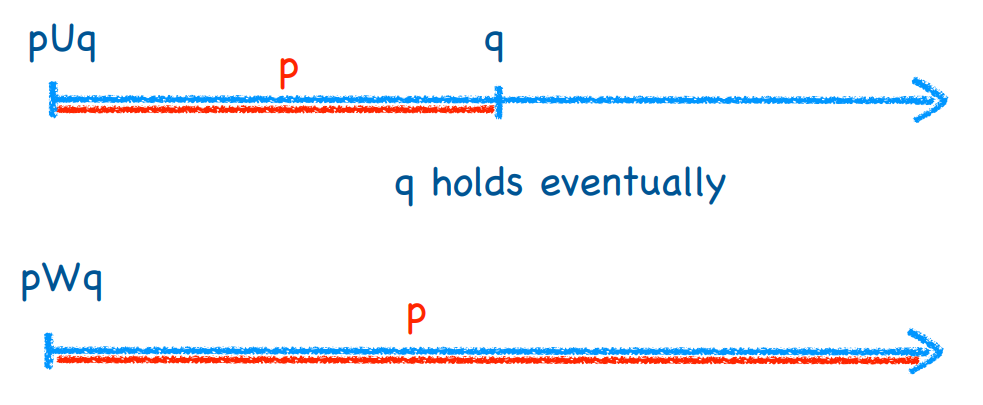
\includegraphics[width=1\textwidth, keepaspectratio]{imgs/strong-weak-until.png}
\caption{Strong and weak until}
\end{figure}
\noindent
There are also two forms for until:
\begin{itemize}
\item \textbf{Strong until} - $q$ must hold eventually in the execution
\item \textbf{Weak until} - $q$ might never hold in the execution, in which case if $p$ holds for the whole execution, weak until still passes.
\end{itemize}

\subsection{Modelling concurrent systems}
\subsubsection{Transition systems}
A transition system is a standard class of models that are used to represent both hardware and software systems. They are used to describe the behaviour of systems. In essence, a transition system is a directed graph where \textbf{nodes} represent states and \textbf{edges} represent transitions. 
\n
\textbf{Atomic propositions} are simple known facts about the states of the system. These are things such as ``$x == 0$" or ``$x < 20$". 

\subsubsection*{Formal definition}
\begin{equation}
TS = (S, Act, T, I, AP, L)
\end{equation}
where
\begin{align*}
S &= \text{set of states} \\
Act &= \text{set of actions} \\
T \subseteq S \times Act \times S &= \text{transition relation} \\
I \subseteq S &= \text{set of initial states} \\
AP &= \text{set of atomic propositions} \\
L:S \rightarrow 2^{AP} &= \text{labelling function} 
\end{align*}
A transition system is called finite if S, Act and AP are finite.
\n
The labelling function is the essential link for proving properties in a transition system.
\begin{equation}
s \models \phi\ \text{iff}\ L(s) \models \phi
\end{equation}

\subsubsection*{Execution fragment}
A \textbf{finite execution fragment} of a transition system is an alternating sequence of states and actions ending with a state. An execution fragment can also be infinite. 
\begin{figure}[H]
\[ \rho = a \xrightarrow[]{\text{getb}} b \xrightarrow[]{\tau} c \xrightarrow[]{\text{getj}} d \]
\caption{Example execution fragment.}
\end{figure}
\noindent
A \textbf{maximal execution fragment} is either finite and ends in a terminal state, or it is infinite. An \textbf{initial execution fragment} starts in an initial state.
\n
An \textit{execution} of a transition system $TS$ is an initial, maximal execution fragment. A state $s$ is called reachable if there is some execution fragment that ends in $s$ and starts in some initial state.

\subsubsection{Data Dependent systems}
Often times executable actions come from conditional branching in systems. To be able to deal with conditionals, conditional transitions can be added to a transition system in the form of a guard. Labels in conditional transitions have the form:
\begin{equation*}
g:\alpha
\end{equation*}
where $g$ is a boolean guard and $\alpha$ is an action that occurs if $g$ holds.
\n
However, a graph containing conditional transitions is \textbf{not} a transition system. To get a transition system from such a graph, it has to be unfolded and additional information added to the state based on the resources it needs. This is where we introduce the concept of program graphs.
\subsubsection{Program graphs}
A program graph over a set \texttt{Var} of typed variables is defined as follows:
\begin{equation}
PG = (Loc, Act, \text{Effect}, C_{\dagger}, Loc_{0}, g_{0})
\end{equation}
where
\begin{align*}
Loc &= \text{set of locations} \\
Act &= \text{set of actions} \\
\text{Effect}:\ Act \times Eval(var) \rightarrow\ Eval(var) &= \text{effect function} \\
C_{\dagger} \subseteq Loc \times Cond(var) \times Act \times Loc &= \text{conditional transition relation} \\
Loc_{0} \subseteq Loc &= \text{set of initial locations} \\
g_{0}\in Cond(Var) &= \text{initial condition}
\end{align*}
\noindent
The \textbf{Effect} indicates how the evaluation $\eta$ of variables is changed by performing an action. For example, if there was a vending machine that spits out beer or juice depending on the action, and we want to keep track of the number of beers and juices in the machine, the effects may look like this:
\begin{align*}
\text{Effect}(\text{getJuice}, \eta)(\text{juiceCount}) &= \eta(\text{juiceCount}) - 1 \\ 
\text{Effect}(\text{getJuice}, \eta)(\text{beerCount}) &= \eta(\text{beerCount}) \\
\text{Effect}(\text{getBeer}, \eta)(\text{juiceCount}) &= \eta(\text{juiceCount}) \\ 
\text{Effect}(\text{getBeer}, \eta)(\text{beerCount}) &= \eta(\text{beerCount}) - 1
\end{align*}
\noindent
The transition system of a program graph - $TS(PG)$ - is the tuple $(S, ACt, T, I, AP, L)$.
\section{Timed automata and UPPAAL}

\subsection{CTL}

\section{Petri nets}




\end{document}
